\documentclass[titlepage,a4paper]{article}

\usepackage{a4wide}
\usepackage[colorlinks=true,linkcolor=black,urlcolor=blue,bookmarksopen=true]{hyperref}
\usepackage{bookmark}
\usepackage{fancyhdr}
\usepackage[spanish]{babel}
\usepackage[utf8]{inputenc}
\usepackage[T1]{fontenc}
\usepackage{graphicx}
\usepackage{float}

\usepackage{minted} %codigo

\pagestyle{fancy} % Encabezado y pie de página
\fancyhf{}
\fancyhead[L]{TP1S - Bruno Grassano}
\fancyhead[R]{Algoritmos y Programación III - FIUBA}
\renewcommand{\headrulewidth}{0.4pt}
\fancyfoot[C]{\thepage}
\renewcommand{\footrulewidth}{0.4pt}
\usepackage[utf8]{inputenc}


\begin{document}
\begin{titlepage} % Carátula
	\hfill
\includegraphics[width=6cm]{logofiuba.jpg}
    \centering
    \vfill
    \Huge \textbf{Trabajo Práctico 1 — Smalltalk}
    \vskip2cm
    \Large [7507/9502] Algoritmos y Programación III\\
    Curso 1 \\ % Curso 1 para el de la tarde y 2 para el de la noche
    Primer cuatrimestre de 2020 
    \vfill
    \begin{tabular}{ | l | l | } % Datos del alumno
      \hline
      Alumno: & Grassano, Bruno \\ \hline
      Número de padrón: & 103855 \\ \hline
      Email: & bgrassano@fi.uba.ar \\ \hline
  	\end{tabular}
    \vfill
    \vfill
\end{titlepage}

\tableofcontents % Índice general
\newpage


%%%%%%%%%%%%%%%%%%%%%%%%%%%%%%%%%%%%%%%%%%%%%%%%%%%%%%%%%%%%%%%%%%


\section{Introducción}\label{sec:intro}
El presente informe reúne la documentación de la solución del primer trabajo práctico de la materia Algoritmos y Programación III que consiste en desarrollar una aplicación de una agencia de pintores en Pharo utilizando los conceptos del paradigma de la orientación a objetos vistos hasta ahora en el curso.


%%%%%%%%%%%%%%%%%%%%%%%%%%%%%%%%%%%%%%%%%%%%%%%%%%%%%%%%%%%%%%%%%%


\section{Supuestos}\label{sec:supuestos}
% Deberá contener explicaciones de cada uno de los supuestos que el alumno haya tenido que adoptar a partir de situaciones que no estén contempladas en la especificación.
El trabajo se realizo con los siguientes supuestos que fueron surgiendo a lo largo de la realizacion del trabajo, ya que estos casos no están contenidos en las especificaciones entregadas.\\
\begin{itemize}
    \item [$*$] El usuario no puede crear un pintor que trabaje con rodillo y pincel a la vez, este trabajara con una sola herramienta. Si se ingresa con el mismo nombre se considera que es otra persona.
    \item [$*$] El usuario sera el encargado de manejar las pinturas que haya creado.
    \item [$*$] El pintor con rodillo no ofrece descuento.
    \item [$*$] El área para el presupuesto tiene sentido lógico, no se pediría un presupuesto para 0 metros cuadrados.
    \item [$*$] Cargar un precio de pintor o pintura como 0 es valido, se considera que se ofrece el servicio o producto gratuitamente.
    \item [$*$] El descuento que ofrecen los pintores es cuando el área a pintar es mayor que 40 metros cuadrados estrictos.
    \item [$*$] El cliente solamente quiere el presupuesto final, es decir, no le interesa como sean las proporciones de este con respecto a la mano de obra y materiales.
\end{itemize}
 
\newpage


%%%%%%%%%%%%%%%%%%%%%%%%%%%%%%%%%%%%%%%%%%%%%%%%%%%%%%%%%%%%%%%%%%


\section{Diagramas de clase}\label{sec:diagramasdeclase}
% Uno o varios diagramas de clases mostrando las relaciones estáticas entre las clases.  Puede agregarse todo el texto necesario para aclarar y explicar su diseño. Recuerden que la idea de todo el documento es que quede documentado y entendible cómo está implementada la solución.

\textit{Se ocultaron los métodos para dar claridad al diagrama al momento de leerlo.}\\
\begin{figure}[H]
\centering
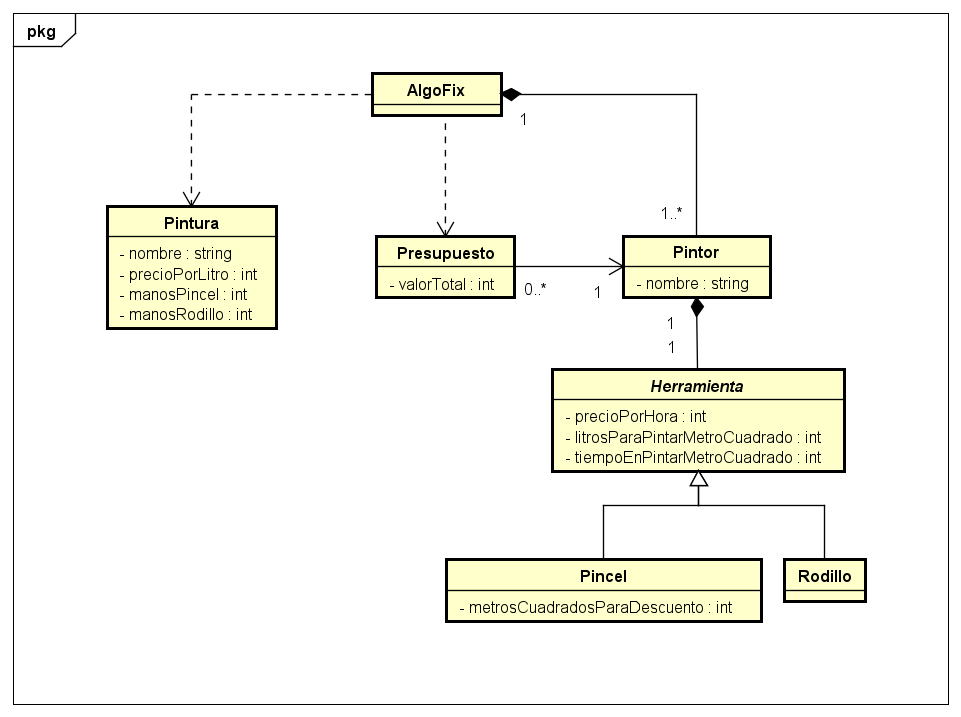
\includegraphics[width=1\textwidth]{Diagrama general.png}
\caption{\label{fig:class04}Diagrama general de la implementación.}
\end{figure}
\indent Este diagrama de clase muestra de forma general la relación que tienen todas las clases del trabajo. Observar que la instancia de AlgoFix va a ser la responsable de realizar las diferentes opciones al ir delegándolas. Notar también que Algofix solamente instancia y utiliza las pinturas, al igual que los presupuestos.

\newpage


\begin{figure}[H]
\centering
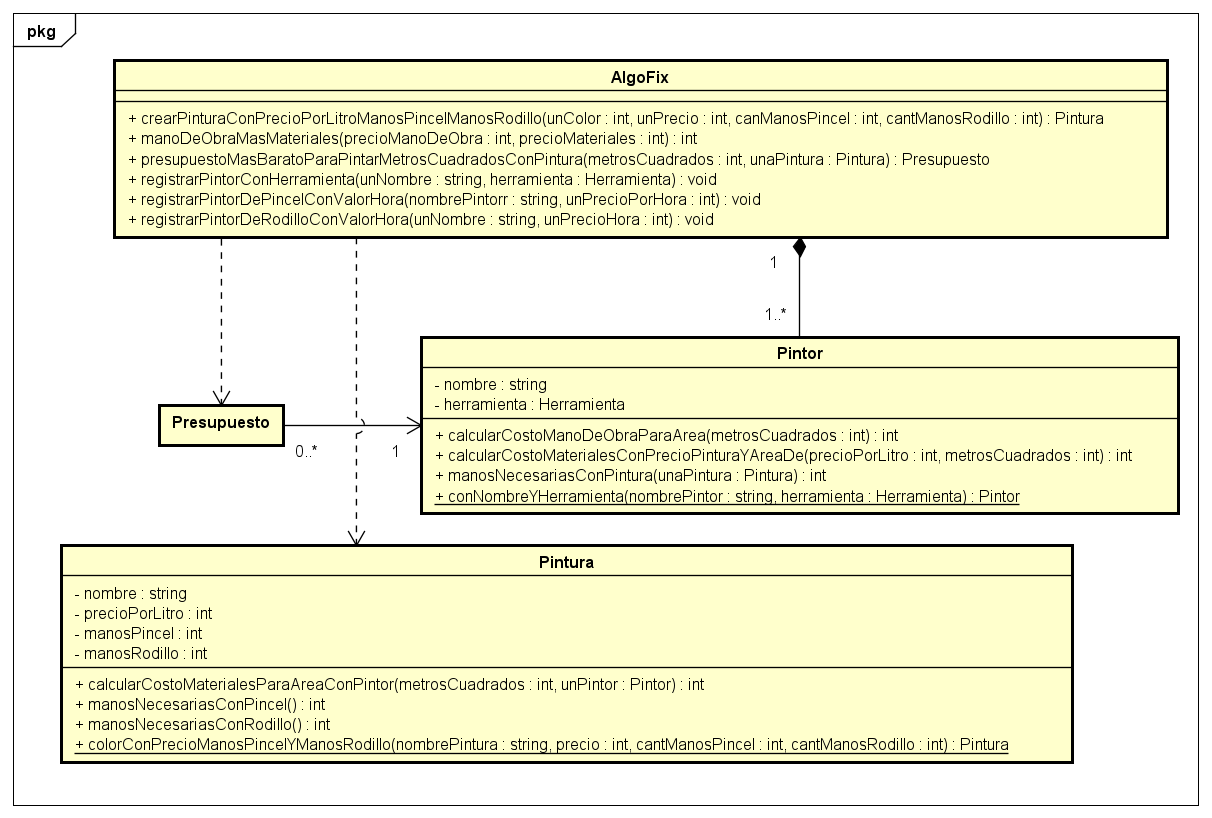
\includegraphics[width=1\textwidth]{AlgoFix.png}
\caption{\label{fig:class01}Diagrama mostrando las relaciones de AlgoFix.}
\end{figure}
En este diagrama se puede observar la relación que tiene AlgoFix con los pintores y las pinturas incluyendo los métodos. Presupuesto solamente se incluyo para indicar la relación que tiene.

\begin{figure}[H]
\centering
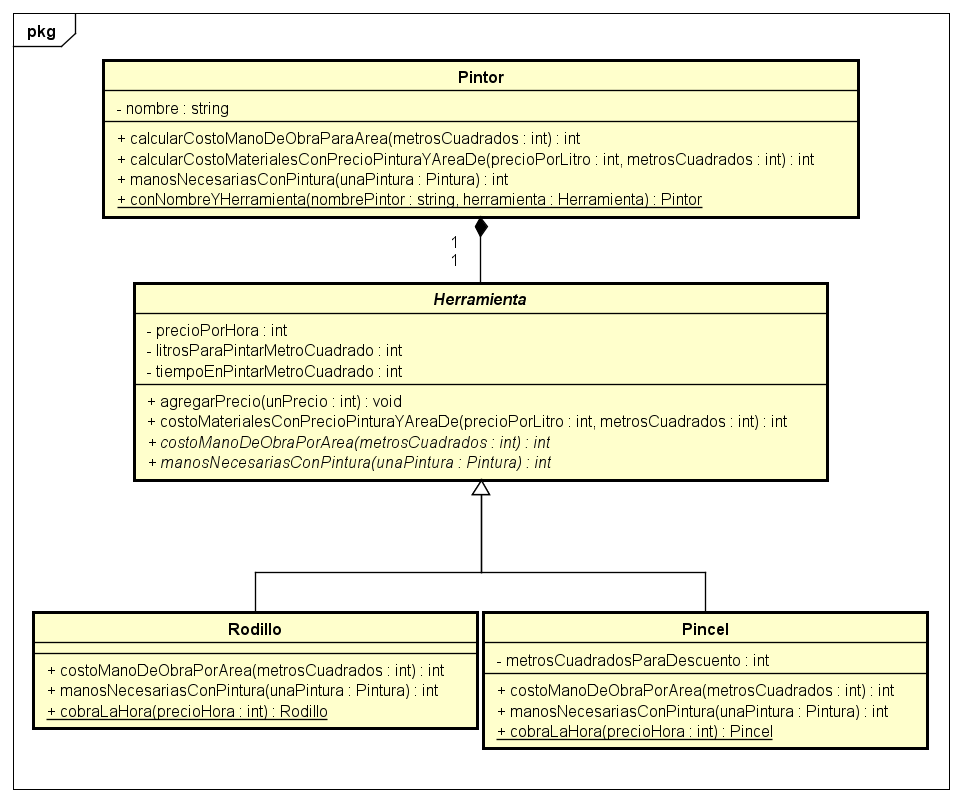
\includegraphics[width=1\textwidth]{Pintor.png}
\caption{\label{fig:class02}Diagrama mostrando en detalle las relaciones del pintor con la herramienta.}
\end{figure}

\begin{figure}[H]
\centering
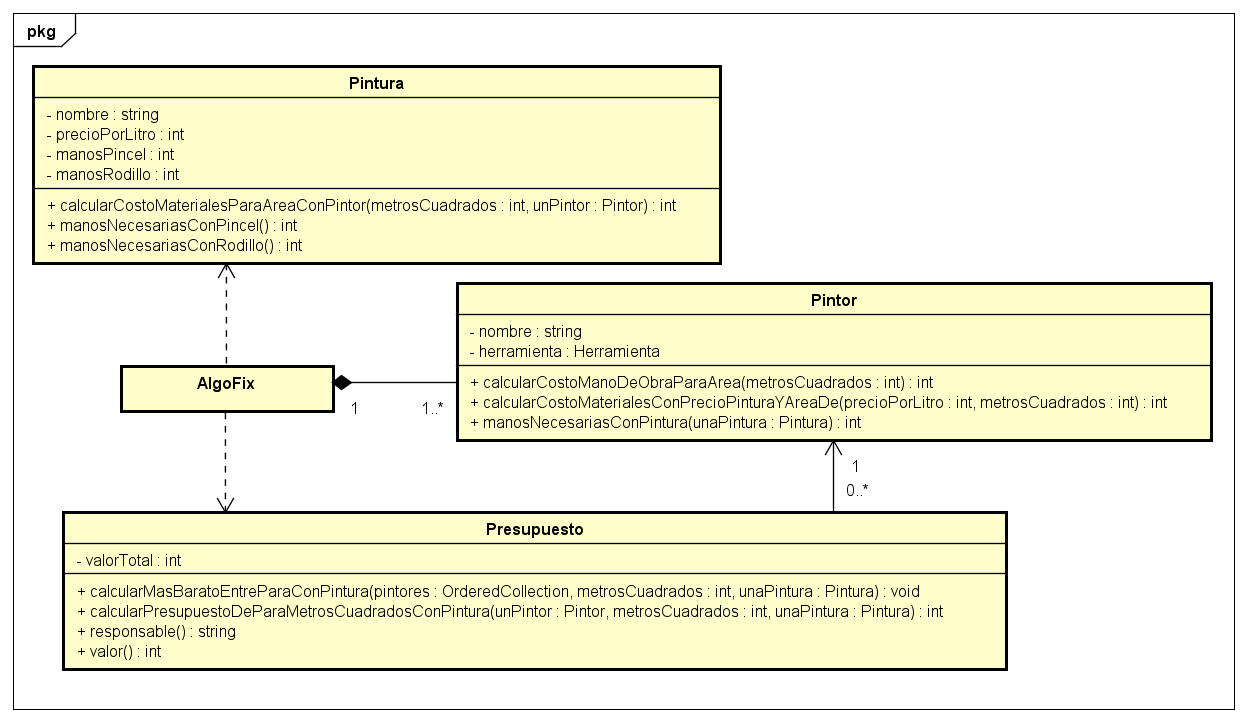
\includegraphics[width=1\textwidth]{Presupuesto.png}
\caption{\label{fig:class03}Diagrama mostrando Presupuesto con sus relaciones.}
\end{figure}
En este diagrama se ocultaron los detalles de AlgoFix junto con algunos métodos de Pintor y Pintura que no son relevantes al momento de realizar un presupuesto.



%%%%%%%%%%%%%%%%%%%%%%%%%%%%%%%%%%%%%%%%%%%%%%%%%%%%%%%%%%%%%%%%%%


\section{Detalles de implementación}\label{sec:implementacion}
% Explicaciones sobre la implementación interna de algunas clases que consideren que puedan llegar a resultar interesantes.

\subsection{AlgoFix}
\indent Esta clase es la responsable general del trabajo, a través de ella se deben de realizar las diferentes opciones disponibles. Internamente como datos solamente almacena una colección de pintores.\\ 
\indent A continuación se detallaran algunos de los métodos mas importantes.\\
\smallskip

\subsubsection*{Método crearPintura:conPrecioPorLitro:manosPincel:manosRodillo:}
\indent Recibe los datos necesarios para crear una pintura. Este metodo le mandara esa información al constructor de Pintura.\\

\subsubsection*{Métodos de registro en AlgoFix}
\indent Estos métodos son  registrarPintorDePincel:conValorHora:,registrarPintorDeRodillo:conValorHora:, y registrarPintor:conHerramienta:.\\
\indent Se encargan de recibir los datos de los pintores con los cuales se va a llamar a los correspondientes constructores. Esto lo hacen primero llamando al constructor de una herramienta, que después es agregada al pintor. El método \textit{registrarPintor:conHerramienta:} es el encargado de finalmente crear el pintor llamando al constructor de este y agregar el pintor a la colección de pintores que tiene AlgoFix. Este método es privado y solamente debería ser usado internamente de AlgoFix. Se muestran a continuación dos de los métodos mencionados.

\begin{minted}{smalltalk}
registrarPintorDePincel: nombrePintor conValorHora: unPrecioPorHora
    self registrarPintor: nombrePintor conHerramienta: (Pincel cobraLaHora: unPrecioPorHora)
\end{minted}

\begin{minted}{smalltalk}
registrarPintor: unNombre conHerramienta: herramienta
    pintores add: (Pintor conNombre: unNombre yHerramienta: herramienta )
\end{minted}

\subsubsection*{Metodo presupuestoMasBaratoParaPintarMetrosCuadrados:conPintura:}
\indent Este método es el que utiliza el usuario para pedir el presupuesto mas barato con la pintura que el indique.
\begin{minted}{smalltalk}
presupuestoMasBaratoParaPintarMetrosCuadrados: metrosCuadrados conPintura: unaPintura
    | presupuesto |
    presupuesto := Presupuesto new.
    presupuesto calcularMasBaratoEntre: pintores para: metrosCuadrados conPintura: unaPintura.
    ^presupuesto
\end{minted}



\subsection{Pintor}
\indent Esta clase almacena los datos del pintor y recibe las instrucciones que vienen de AlgoFix o Presupuesto. \\
\indent Como variables de instancia posee el nombre y una herramienta. La elección de utilizar una herramienta para abstraer parte de su comportamiento se debe a que facilita y vuelve mas claras las operaciones correspondientes a los cálculos. Una ventaja adicional de esto, es que si se quisiera se podrían implementar varias herramientas distintas, o incluso crear un pintor que pueda trabajar con rodillo y pincel a la vez. Lo único necesario para que esto suceda es que esas herramientas entiendan los mismos mensajes. En su apartado se explicara con mas detalle esta decisión de usar herencia con polimorfismo\\
\indent A continuación se muestran los métodos correspondientes a esta clase.
\medskip

\subsubsection*{Métodos obtenerNombre,agregarNombre:, y agregarHerramienta:}
\indent Estos métodos son utilizados durante la creación de un pintor, o durante el pedido de información relevante para el cliente, este es el caso del nombre. Estos métodos son privados y no deberían ser usados desde afuera.
\medskip

\subsubsection*{Métodos calcularCostoManoDeObraParaArea: y calcularCostoMaterialesConPrecioPintura:yAreaDe:}
\indent Estos métodos reciben los metros cuadrados y un precio en el caso de \textit{calcularCostoMaterialesConPrecioPintura:yAreaDe:}. Se encargan de delegar en la herramienta los cálculos necesarios para obtener las partes del presupuesto. Ambos precios que devuelva no contendrán el valor de la cantidad de manos necesarias para el trabajo. Esto es agregado en otro momento, ya que se saco como factor común en la cuenta porque no es necesario en ese momento conocer la cantidad de manos. Haciendo esto se ahorra estar enviándole un parámetro más a los mensajes,evitando que se termine complicando un poco la lectura del código.\\

\begin{minted}{smalltalk}
calcularCostoManoDeObraParaArea: metrosCuadrados	
    ^herramienta costoManoDeObraPorArea: metrosCuadrados 
\end{minted}

\begin{minted}{smalltalk}
calcularCostoMaterialesConPrecioPintura: precioPorLitro yAreaDe: metrosCuadrados
    ^herramienta costoMaterialesConPrecioPintura: precioPorLitro  yAreaDe: metrosCuadrados    
\end{minted}
\medskip

\subsubsection*{Método manosNecesariasConPintura:}
\indent Este método también delega en la herramienta el saber cuantas manos son necesarias con la pintura que le manden. \\
\indent Al comienzo se encontró el problema que había que encontrar una forma de poder tener la cantidad de manos necesarias de la pintura, por lo que se implemento temporalmente una estructura de control que terminaba rompiendo el encapsulamiento de las herramientas. Finalmente se decidió arreglar el problema de esta forma ya que así no es necesario saber que herramienta es realmente la que tiene el pintor. La herramienta misma, como veremos mas adelante, le pregunta a la pintura cuantas manos necesita para si misma al utilizar polimorfismo.
\begin{minted}{smalltalk}
manosNecesariasConPintura: unaPintura
    ^herramienta manosNecesariasConPintura: unaPintura
\end{minted}


\subsection{Herramienta, Rodillo y Pincel}
Al comienzo del trabajo, este estaba siendo implementado con dos clases de pintores, siendo estas \textit{PintorConRodillo y PintorConPincel}. Pero llegado el momento de refactorización se llego a observar que iba a ser mas claro tener una clase \textit{Pintor} que tenga un \textit{Pincel o Rodillo}. \\
\indent Al estar implementándolas, se vio que compartían bastante código resultando en codigo repetido, por lo que se llego a la conclusión que era mejor abstraer la parte en donde diferían, siendo esta la idea del instrumento del pintor. Por lo tanto, se creo una clase abstracta llamada \textit{Herramienta}, de la cual heredarían \textit{Pincel y Rodillo}, ya que estas clases cumplen la relación ''es un'' con la herramienta. Esta decisión de diseño termino brindando mas facilidad y claridad, ya que solamente fue necesario implementar los dos métodos en donde diferían \textit{Pincel y Rodillo}.\\
\indent La clase Herramienta contiene como variables de instancia litrosParaPintarMetroCuadrado y tiempoEnPintarMetroCuadrado, estas variables son inicializas y utilizadas como constantes durante la ejecución.
\medskip

\subsubsection*{Método de clase cobraLaHora:}
\indent Este método de clase esta implementado en \textit{Pincel y Rodillo}, vendrían a ser los constructores de las herramientas.\\
\indent Se eligió ese nombre ya que esta pensado para que durante la creación de los pintores se lea todo junto. Un ejemplo de esto se puede ver en el apartado correspondiente a AlgoFix en la parte de los registros de pintores.\\
\indent Este constructor creara la herramienta pedida y utilizara el setter agregarPrecio:.
Este setter es privado y no debería ser usado desde afuera.\\
\medskip

\subsubsection*{Método costoManoDeObraPorArea:}
\indent Este mensaje esta implementado y es responsabilidad de las clases hijas \textit{Pincel y Rodillo}. Su responsabilidad es el el calculo de la mano de obra sin aplicar el costo de las manos. \\
\indent A continuación se muestra primero el código correspondiente a la clase Pincel y después el de Rodillo. Observar que la diferencia esta principalmente en el descuento que se puede aplicar con pincel, resultando en un método ligeramente mas largo. Esto se debe a la estructura de control utilizada para determinar si corresponde un descuento. A este ''if''  no se le encontró una forma clara de poder evitarlo.
\newpage
\begin{minted}{smalltalk}
costoManoDeObraPorArea: metrosCuadrados
    | descuento |
    (metrosCuadrados <= 0) ifTrue:[AreaDebeSerMayorACeroError new signal.].
    descuento := 1.
    (metrosCuadradosParaDescuento < metrosCuadrados )ifTrue: [  
        descuento := 0.5.
    ].
    ^precioPorHora * metrosCuadrados * tiempoEnPintarMetroCuadrado * descuento
\end{minted}

\begin{minted}{smalltalk}
costoManoDeObraPorArea: metrosCuadrados
    (metrosCuadrados <= 0) ifTrue:[AreaDebeSerMayorACeroError new signal.].
    ^precioPorHora * metrosCuadrados  * tiempoEnPintarMetroCuadrado
\end{minted}

\medskip
\subsubsection*{Método costoMaterialesConPrecioPintura}
\indent Esta implementado en la clase herramienta y es heredado por las clases hijas. El comportamiento es igual en ambas.

\begin{minted}{smalltalk}
costoMaterialesConPrecioPintura: precioPorLitro yAreaDe: metrosCuadrados
    (metrosCuadrados <= 0)ifTrue:[AreaDebeSerMayorACeroError new signal].
    ^precioPorLitro * metrosCuadrados * litrosParaPintarMetroCuadrado 
\end{minted}

\medskip
\subsubsection*{Método manosNecesariasConPintura:}
\indent Le pregunta a la pintura cuantas manos son necesarias para la herramienta que la esta llamando. Se aprovecho enormemente el polimorfismo en este caso, ya que implementar este mensaje fue la forma de evitar romper el encapsulamiento de las herramientas preguntadoles directamente que tipo de herramienta eran.

\begin{minted}{smalltalk}
manosNecesariasConPintura: unaPintura
    ^unaPintura manosNecesariasConPincel
\end{minted}

\begin{minted}{smalltalk}
manosNecesariasConPintura: unaPintura
    ^unaPintura manosNecesariasConRodillo
\end{minted}


\subsection{Pintura}
\indent Las instancias de esta clase son creadas por AlgoFix y son manejadas por los clientes. Contiene toda la información relevante de una pintura y es utilizada para calcular parte de los presupuestos.


\subsubsection*{Método de clase color:conPrecio:manosPincel:yManosRodillo:}
\indent Es el constructor que utilizan las pinturas. Este al crearlas utiliza varios setters que son privados y no deberían ser usados desde afuera. Estos métodos son \emph{agregarNombre:}, \emph{agregarPrecio:}, \emph{agregarManosPincel:}, y \emph{agregarManosRodillo:}.

\medskip

\subsubsection*{Métodos manosNecesariasConRodillo y manosNecesariasConPincel}
Simplemente devuelven el dato pedido a la pintura.


\medskip

\subsubsection*{Método calcularCostoMaterialesParaArea:}
Delega en el pintor el calculo correspondiente a los materiales, pasando la informacion del precio de la pintura.
\begin{minted}{smalltalk}
calcularCostoMaterialesParaArea: metrosCuadrados conPintor: unPintor
    ^ unPintor calcularCostoMaterialesConPrecioPintura: precioPorLitro
        yAreaDe: metrosCuadrados     
\end{minted}

\subsection{Presupuesto}
\indent Esta clase esta ya que es una de las pedidas por el enunciado. Se encarga de administrar las operaciones generales de buscar el mejor presupuesto para la cantidad de metros cuadrados indicada. Internamente guarda al pintor que ofrece el mejor presupuesto y al valor total de este.

\subsubsection*{Métodos valor y responsable}
\indent Pedidos en las pruebas provistas por la cátedra, devuelven los datos correspondientes al presupuesto.

\medskip

\subsubsection*{Método calcularMasBaratoEntre:para:conPintura:}
\indent Este método se encarga de la búsqueda del pintor que ofrezca el menor presupuesto, para eso, se llama a si mismo con el mensaje \textit{calcularPresupuestoDe:paraMetrosCuadrados:conPintura:} que va a ser el responsable de calcular el presupuesto correspondiente a cada pintor. \\
\indent Luego de finalizar la búsqueda, se decidió realizar el calculo devuelta para el mejor pintor ya que este valor no queda guardado durante el proceso anterior. No se quiso realizar el calculo al momento de pedir el valor ya que en ese caso no se tiene la pintura para realizar las cuentas.

\begin{minted}{smalltalk}
calcularMasBaratoEntre: pintores para: metrosCuadrados conPintura: unaPintura
    (pintores isEmpty)ifTrue:[NoHayPintoresRegistradosError new signal].
    pintorConMejorPresupuesto := pintores detectMin: [ :unPintor | 
        self calcularPresupuestoDe: unPintor paraMetrosCuadrados: metrosCuadrados 
            conPintura: unaPintura.
    ].
    valorTotal := self calcularPresupuestoDe: pintorConMejorPresupuesto 
                paraMetrosCuadrados: metrosCuadrados conPintura: unaPintura.
\end{minted}

\subsubsection*{Método calcularPresupuestoDe:paraMetrosCuadrados:conPintura:}
\indent Este método divide en tres partes el calculo del presupuesto de cada pintor.
La primera parte corresponde al calculo de la mano de obra, es decir, el precio que corresponde al pintor por realizar el trabajo. La segunda parte corresponde a los materiales, por lo que se necesita de la pintura y de la herramienta con la que trabaje el pintor. Finalmente , la tercera parte es multiplicar por la cantidad de manos necesarias para pintar. Esto se realiza al final ya que se vio que se simplificaba y evitaba estar pasando un parámetro más a los diferentes métodos del pintor.

\begin{minted}{smalltalk}
calcularPresupuestoDe: unPintor paraMetrosCuadrados: metrosCuadrados conPintura: unaPintura
    | valorManoDeObra valorMateriales presupuesto |
    valorManoDeObra := unPintor calcularCostoManoDeObraParaArea: metrosCuadrados.
    valorMateriales := unaPintura calcularCostoMaterialesParaArea: metrosCuadrados 
                      conPintor: unPintor.

    presupuesto := (valorManoDeObra + valorMateriales) * 
                    (unPintor manosNecesariasConPintura: unaPintura).
	
    ^presupuesto
\end{minted}


%%%%%%%%%%%%%%%%%%%%%%%%%%%%%%%%%%%%%%%%%%%%%%%%%%%%%%%%%%%%%%%%%%

\section{Excepciones}\label{sec:excepciones}
% Explicación de cada una de las excepciones creadas y con qué fin fueron creadas.

\begin{description}
\item[NoHayPintoresRegistradosError] Esta excepción fue creada con el objetivo de evitar problemas en caso de que el usuario intente realizar la operación \textit{presupuestoMasBaratoParaPintarMetrosCuadrados:conPintura:} cuando la instancia de AlgoFix llamada no tiene ningún pintor registrado.
\item[PrecioNoPuedeSerNegativoError] Esta excepción cumple el objetivo de evitar que el usuario ingrese algún precio negativo, ya sea en pinturas o en el precio del pintor. Si esto estuviese permitido, no tendrían sentido los diferentes costos.
\item[AreaDebeSerMayorACeroError] Esta excepción indica que el usuario intento pedir un presupuesto con una cantidad de metros cuadrados nula o negativa. Esto no tendría sentido al momento de realizar los diferentes cálculos.
\item[LaCantidadDeManosDebeSerMayorACeroError] Esta excepción se lanza cuando se intenta crear una pintura con cero o menos manos de pintura, ya sea en rodillos o pincel. Ya que por lo menos algo de pintura se le debe de pasar a la superficie pintada.
\item[PresupuestoNoCalculadoError] Esta excepción fue creada para que se lance cuando se le pide a un presupuesto el responsable o el valor cuando por algún motivo no se tiene uno.
\end{description}


%%%%%%%%%%%%%%%%%%%%%%%%%%%%%%%%%%%%%%%%%%%%%%%%%%%%%%%%%%%%%%%%%%


\section{Diagramas de secuencia}\label{sec:diagramasdesecuencia}
% Mostrar las secuencias interesantes que hayan implementado. Pueden agregar texto para explicar si algo no queda claro.

\begin{figure}[H]
\centering
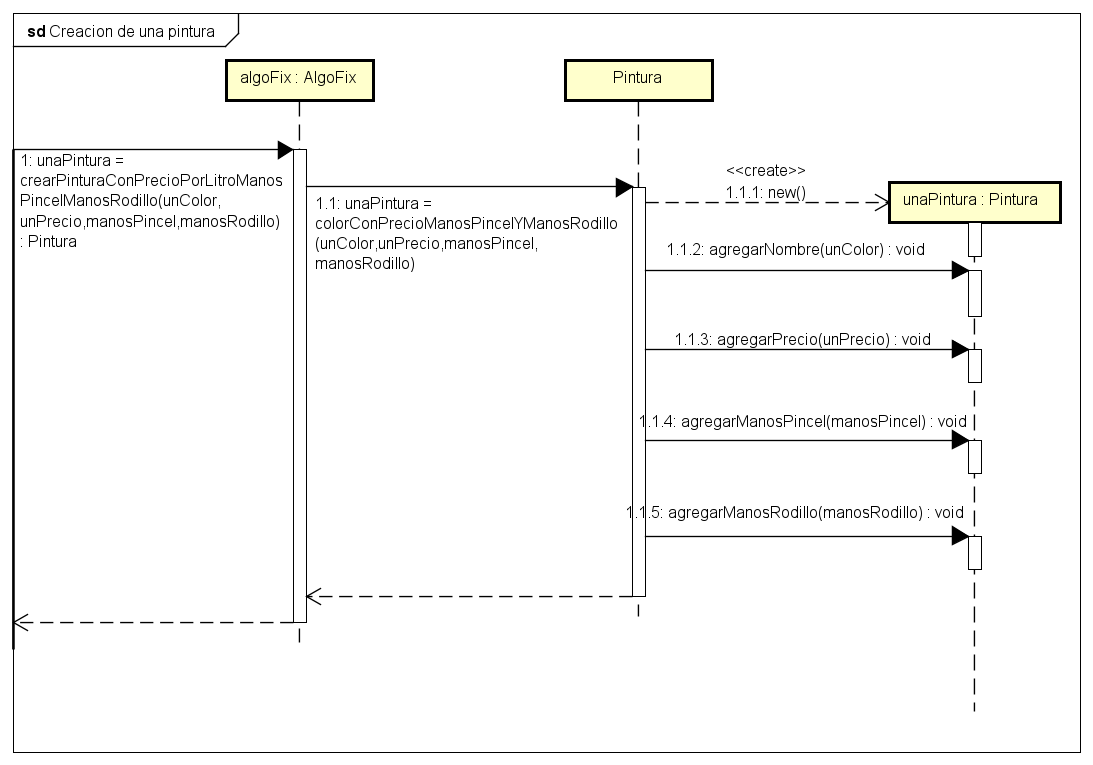
\includegraphics[width=1\textwidth]{Creacion de una pintura.png}
\caption{\label{fig:seq04}Creación de las pinturas}
\end{figure}


\begin{figure}[H]
\centering
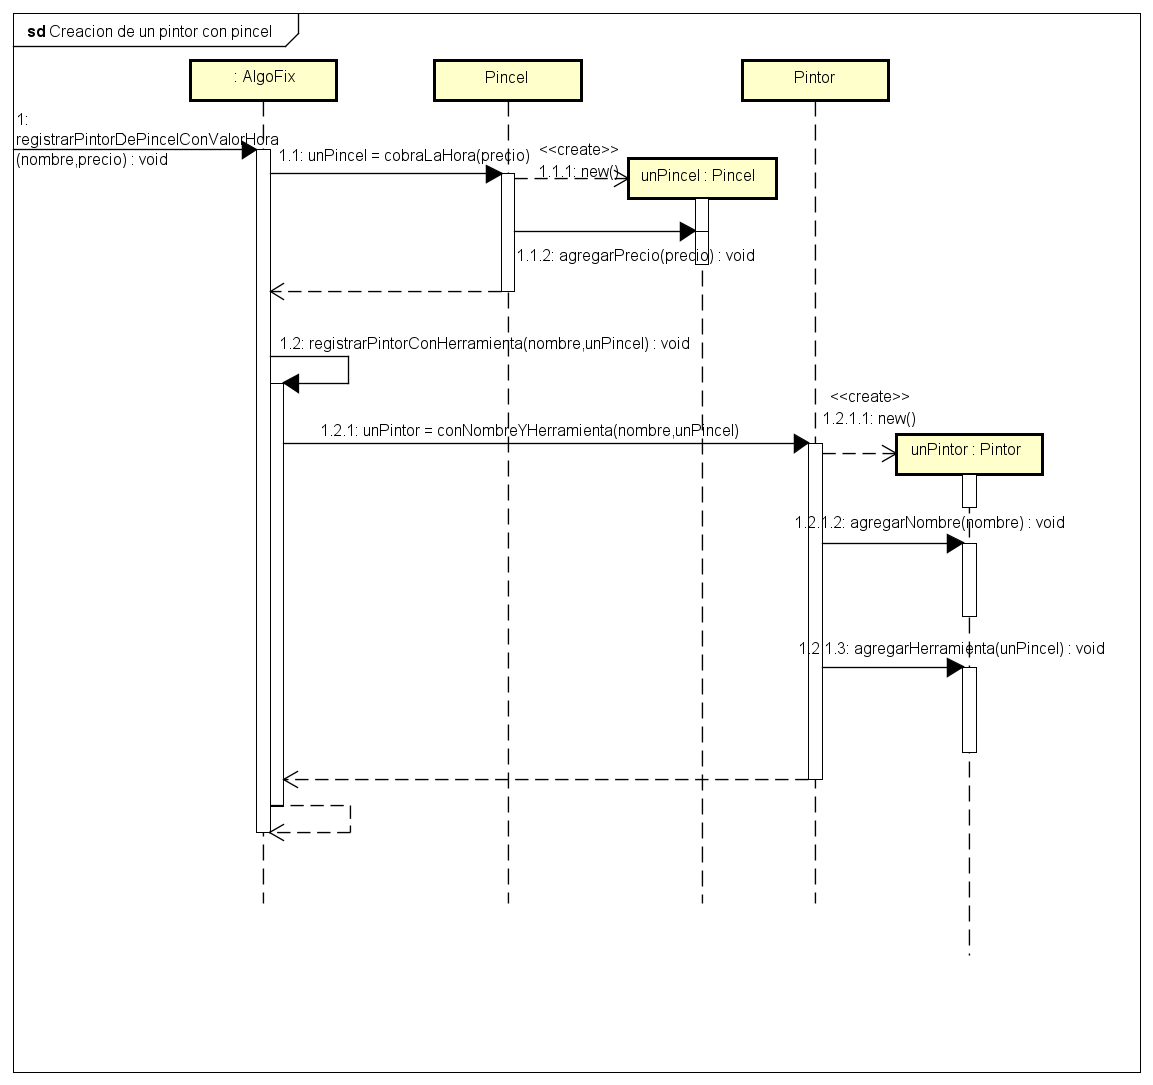
\includegraphics[width=1\textwidth]{Creacion de un pintor con pincel.png}
\caption{\label{fig:seq05}Creación de pintor con pincel}
\end{figure}
\indent En el caso de querer crear un pintor con rodillo seria muy similar, solamente cambia la clase que recibe el mensaje de creación y la instancia creada.

\begin{figure}[H]
\centering
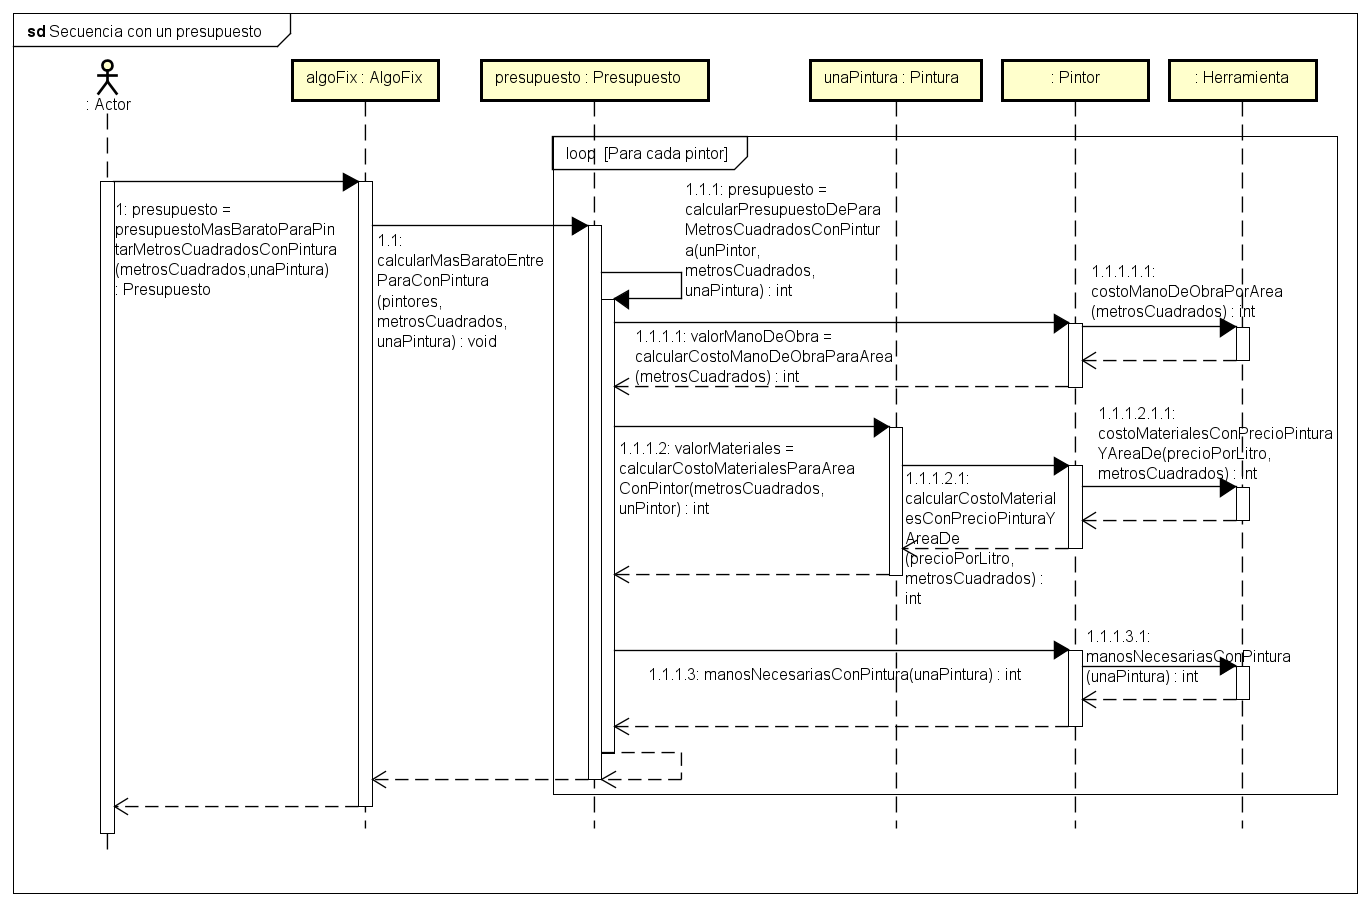
\includegraphics[width=1.1\textwidth]{Secuencia con un presupuesto.png}
\caption{\label{fig:seq03}Calculo de un presupuesto.}
\end{figure}
\indent Se omitió en el diagrama el mensaje <<create>> que iría de algoFix a la clase de presupuesto para que quede mas prolijo. 
\begin{figure}[H]
\centering
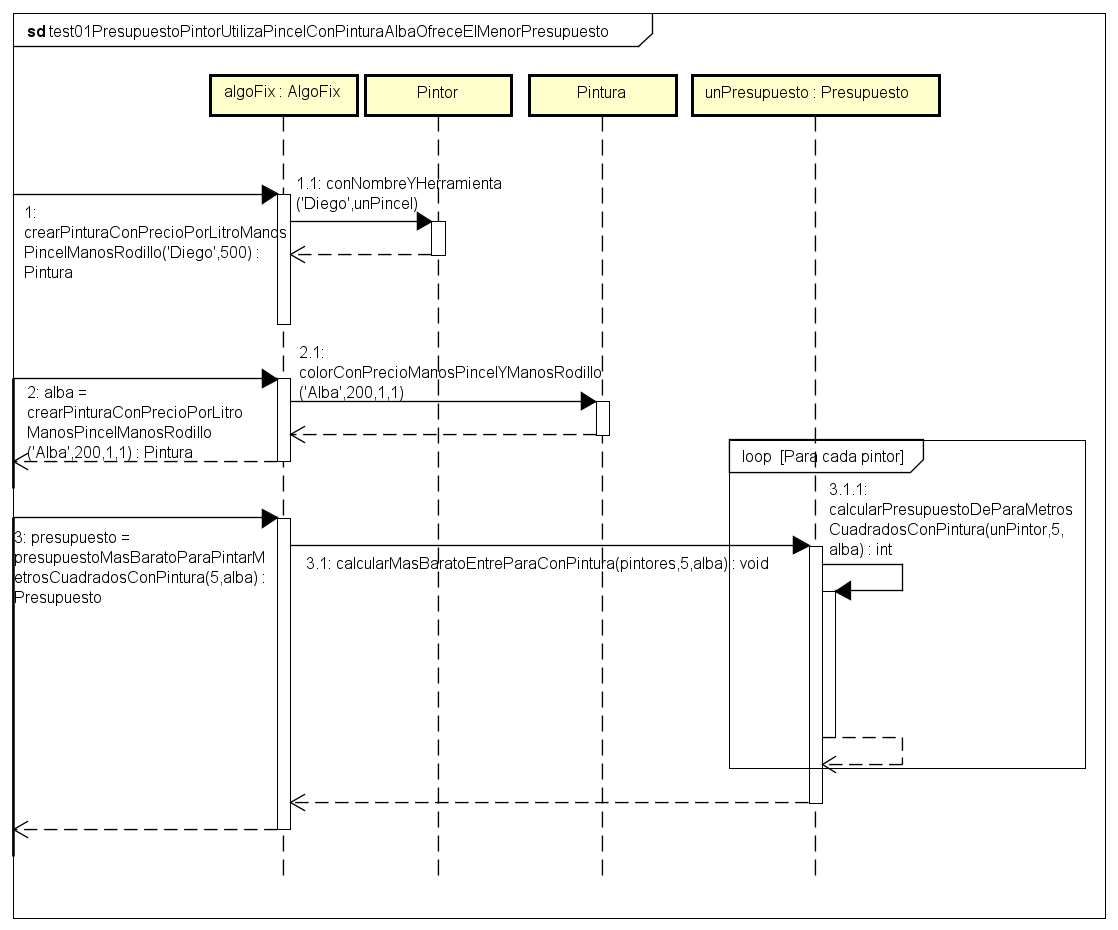
\includegraphics[width=1\textwidth]{test01PresupuestoPintorUtilizaPincelConPinturaAlbaOfreceElMenorPresupuesto.png}
\caption{\label{fig:seq01}Prueba 01 provista por la cátedra}
\end{figure}
\indent Este diagrama muestra la primera prueba del trabajo. Como se puede ver, se crea un solo pintor y una pintura. Luego se le pide a algoFix el presupuesto más barato, el cual terminara siendo el del único pintor cargado. \\
\indent Se ocultaron algunos métodos internos para dar mas claridad al diagrama. Estos detalles internos fueron mostrados en los diagramas anteriores.

\begin{figure}[H]
\centering
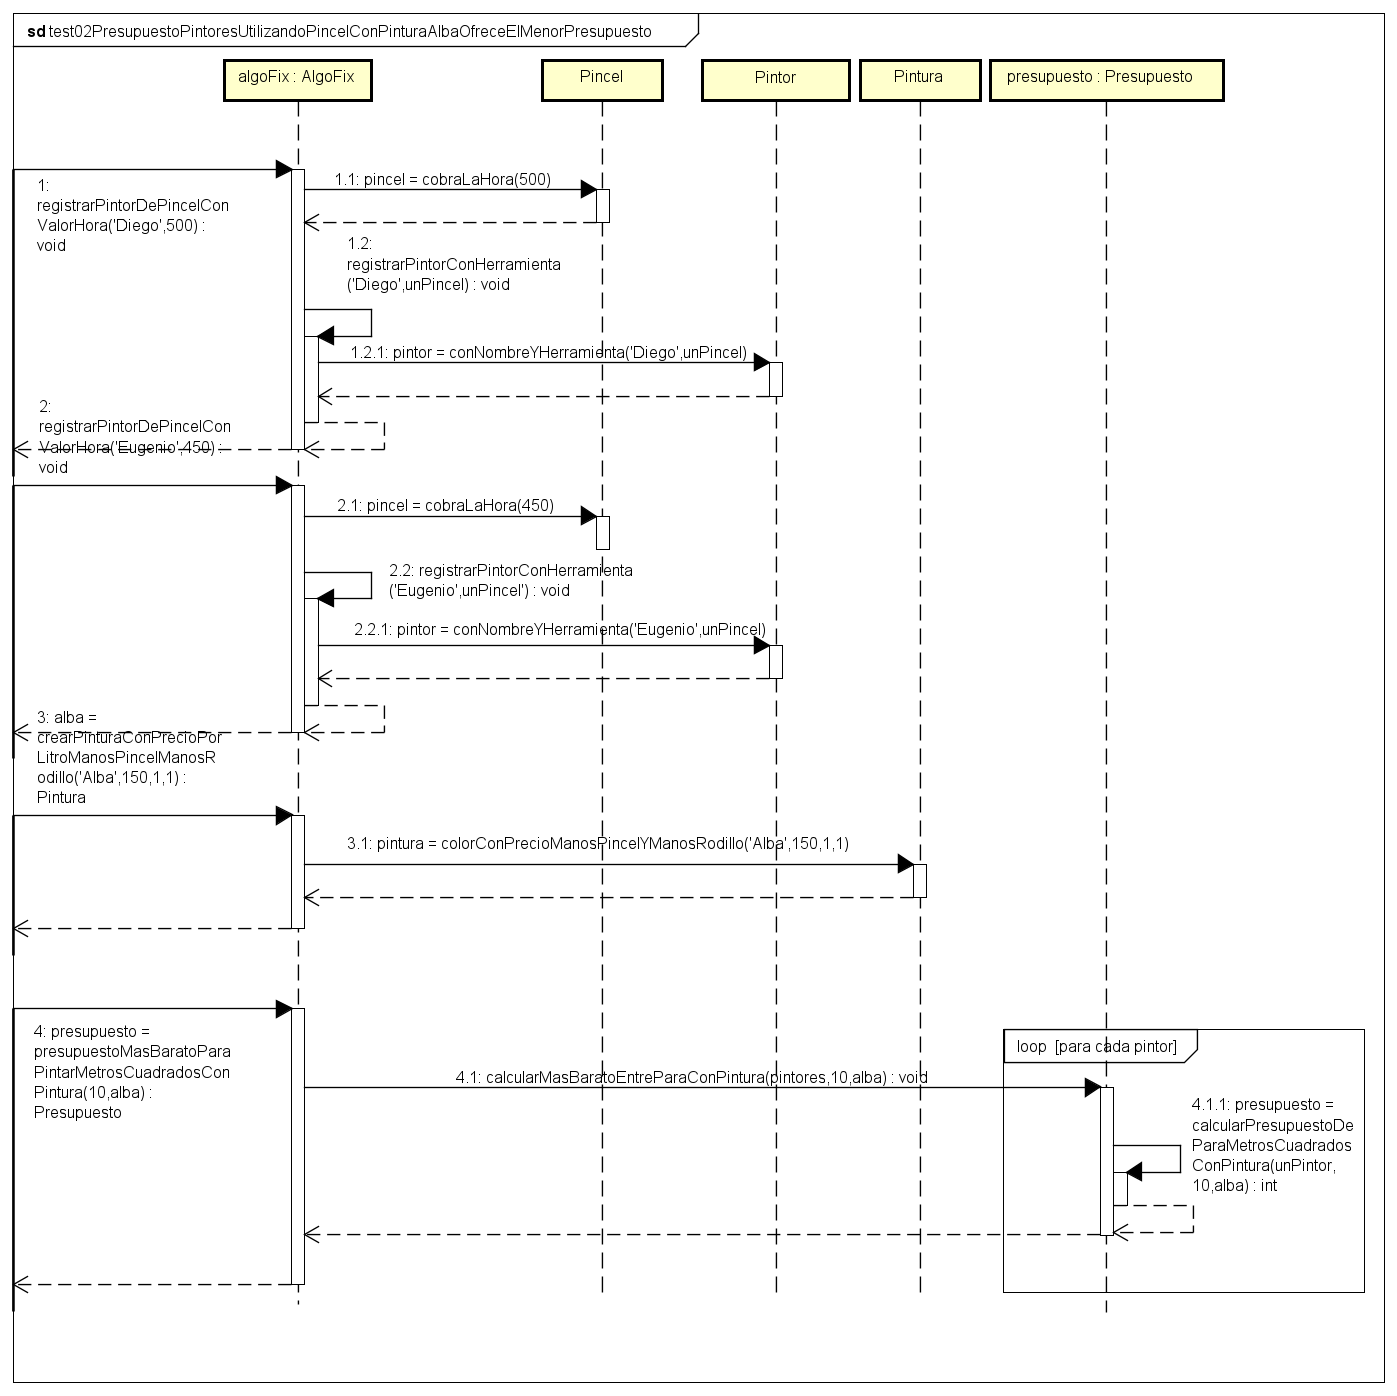
\includegraphics[width=1\textwidth]{test02PresupuestoPintoresUtilizandoPincelConPinturaAlbaOfreceElMenorPresupuesto.png}
\caption{\label{fig:seq02}Prueba 02 provista por la cátedra}
\end{figure}

En este diagrama se puede observar la segunda prueba provista por la cátedra. Los partes que surgen de los dos primeros llamados a algoFix corresponden al agregado de los pintores con pincel a la colección que esta contiene. Estos pintores son 'Diego' y 'Eugenio'. \\
\indent La tercera parte responde a la creación de la pintura que pide el usuario, en este caso la pintura 'alba'. Por ultimo, la cuarta parte es el pedido de un presupuesto para 10 metros cuadrados.
Este presupuesto seria creado en algoFix y se le es mandado el mensaje para que calcule el mas barato. Este luego recorrerá cada pintor en la colección que recibe y se quedara con el que menor presupuesto tenga.\\
\indent En este diagrama de clases, se ocultaron algunos métodos que no se vieron necesarios para transmitir el objetivo de la prueba. Estos son algunos setters y getters junto con los mensajes internos del presupuesto para el calculo. Esto se puede ver en los anteriores diagramas.


\end{document}
